\chapter*{Dodatak: Prikaz aktivnosti grupe}
		\addcontentsline{toc}{chapter}{Dodatak: Prikaz aktivnosti grupe}
		
		\section*{Dnevnik sastajanja}
		
		%\textbf{\textit{Kontinuirano osvježavanje}}\\
		
		 %\textit{U ovom dijelu potrebno je redovito osvježavati dnevnik sastajanja prema predlošku.}
		
		\begin{packed_enum}
			\item  sastanak
			
			\item[] \begin{packed_item}
				\item Datum: 18. listopada 2023.
				\item Prisustvovali: T. Pranjić, J. Mihelčić, A. Mesić, D. Mišetić, A. Sorić, I. Ćorluka, N. Perić
				\item Teme sastanka:
				\begin{packed_item}
					\item Formiranje tima
					\item Odabir voditelja
				\end{packed_item}
			\end{packed_item}
			
			\item  sastanak
			\item[] \begin{packed_item}
				\item Datum: 25. listopada 2023.
				\item Prisustvovali: T. Pranjić, J. Mihelčić, A. Mesić, D. Mišetić, A. Sorić, I. Ćorluka, N. Perić
				\item Teme sastanka:
				\begin{packed_item}
					\item  Razjašnjavanje pojedinosti oko projektnog zadatka

				\end{packed_item}
			\end{packed_item}
      
      \item  sastanak
			\item[] \begin{packed_item}
			  \item Datum: 25. listopada 2023.
				\item Prisustvovali: A. Sorić, D. Mišetić
				\item Teme sastanka:
				\begin{packed_item}
					\item  Opis projektnog zadatka
        \end{packed_item}
     \end{packed_item}
			
	  \item  sastanak
			\item[] \begin{packed_item}
			  \item Datum: 08. siječnja 2024.
				\item Prisustvovali:  T. Pranjić, J. Mihelčić, A. Mesić, D. Mišetić, A. Sorić, I. Ćorluka, N. Perić
				\item Teme sastanka:
				\begin{packed_item}
					\item  Plan rada za drugi ciklus
        \end{packed_item}
	\end{packed_item}

		%
 
		\end{packed_enum}
		
		\eject
		\section*{Tablica aktivnosti}
		
			%\textbf{\textit{Kontinuirano osvježavanje}}\\
			
			 %\textit{Napomena: Doprinose u aktivnostima treba navesti u satima po članovima grupe po aktivnosti.}

			\begin{longtblr}[
					label=none,
				]{
					vlines,hlines,
					width = \textwidth,
					colspec={X[7, l]X[1, c]X[1, c]X[1, c]X[1, c]X[1, c]X[1, c]X[1, c]}, 
					vline{1} = {1}{text=\clap{}},
					hline{1} = {1}{text=\clap{}},
					rowhead = 1,
				} 
			
\SetCell[c=1]{c}{} & \SetCell[c=1]{c}{\rotatebox{90}{\textbf{Tomislav Pranjić}}} & \SetCell[c=1]{c}{\rotatebox{90}{\textbf{Ante Sorić}}} &	\SetCell[c=1]{c}{\rotatebox{90}{\textbf{Diego Mišetić}}} & \SetCell[c=1]{c}{\rotatebox{90}{\textbf{Josip Mihelčić}}} &	\SetCell[c=1]{c}{\rotatebox{90}{\textbf{Antonia Mesić}}} & \SetCell[c=1]{c}{\rotatebox{90}{\textbf{Ivan Ćorluka}}} &	\SetCell[c=1]{c}{\rotatebox{90}{\textbf{Nikola Perić}}} \\  

         			Upravljanje projektom 			            & 10 &  &  & 8 &  &  & \\ 
				Opis projektnog zadatka 	              &  & 8 & 8 &  &  &  & \\
				Funkcionalni zahtjevi       		          &  &  &  &  &  &  & 8 \\ 
				Opis pojedinih obrazaca 		          & 1 &  &  & 2 &  &  &  \\ 
				Dijagram obrazaca 				             & 3 &  &  & 3 &  &  &  \\ 
				Sekvencijski dijagrami 				        &  &  & 6 &  &  &  &  \\ 
				Opis ostalih zahtjeva 				          &  &  &  &  &  & 2  &  \\ 
				Arhitektura i dizajn sustava	          & 2 &  &  &  &  &  & 1  \\ 
				Baza podataka						  			& 3 &  & 3 &  &  &  &   \\ 
				Dijagram razreda 					 		   &  & 5 &  & 2 &  &  &   \\  
				Dijagram stanja						   	         &  &  & 6 &  &  &  &  \\ 
				Dijagram aktivnosti 				  	      &  &  & 5 &  &  &  &  \\ 
				Dijagram komponenti				 	       &  &  & 5 &  &  &  &  \\ 
				Korištene tehnologije i alati 	 	       & 2 &  &  &  &  &  &  \\ 
				Ispitivanje programskog rješenja 	& 6 &  &  &  &  &  &  \\ 
				Dijagram razmještaja						&  &  & 5 &  &  &  &  \\ 
				Upute za puštanje u pogon 			   & 4 &  &  &  &  &  &  \\  
				Dnevnik sastajanja 			                  &  &  &  &  &  &  &  \\ 
				Zaključak i budući rad 		                 & 2 &  &  &  &  &  &  \\  
				\textit{Backend: Generičke funkcionalnosti i sigurnost} 			&  & 16 &  & 18 &  &  &  \\ 
				\textit{Frontend: Izrada početne stranice} 				&  &  &  &  &  &  & 8 \\
				\textit{Frontend: Izrada stranice za upravljanje prijevoznikom}     &  &  &  &  &  &  & 17 \\ 
				\textit{Frontend: Izrada stranice za upravljanje smještajem}	    &  &  &  &  &  14  & & \\
				\textit{Frontend: Izrada stranice za upravljanje korisnicima}	    &  &  &  &  & & 16 & \\
				\textit{Baza podataka: Izrada baze podataka} 		 			& 4 &  &  &  &  &  & \\  
				\textit{Frontend: Izrada stranice za prijavu}             &  &  &  &  &  &  & 9 \\ 
				\textit{Baza podataka: Izrada baze podataka} 		 		& 4 &  &  &  &  &  & \\  
				\textit{Backend: Spajanje s bazom podataka} 				&  &  &  & 8 &  &  &  \\ 
				\textit{Backend: Implementacija funkcionalnosti}			&  & 15 &  & 30 &  &  &  \\
				\textit{Backend: Povezivanje s frontendom}					&  &  &  & 30 &  &  &  \\
				\textit{Puštanje sustava u pogon}							& 20 &  &  & 15 &  &  &\\
			\end{longtblr}
					
					
		\eject
		\section*{Dijagrami pregleda promjena}
		
		%\textbf{\textit{dio 2. revizije}}\\
		
		%\textit{Prenijeti dijagram pregleda promjena nad datotekama projekta. Potrebno je na kraju projekta generirane grafove s gitlaba prenijeti u ovo poglavlje dokumentacije. Dijagrami za vlastiti projekt se mogu preuzeti s gitlab.com stranice, u izborniku Repository, pritiskom na stavku Contributors.}
		
		\begin{figure}[H]
			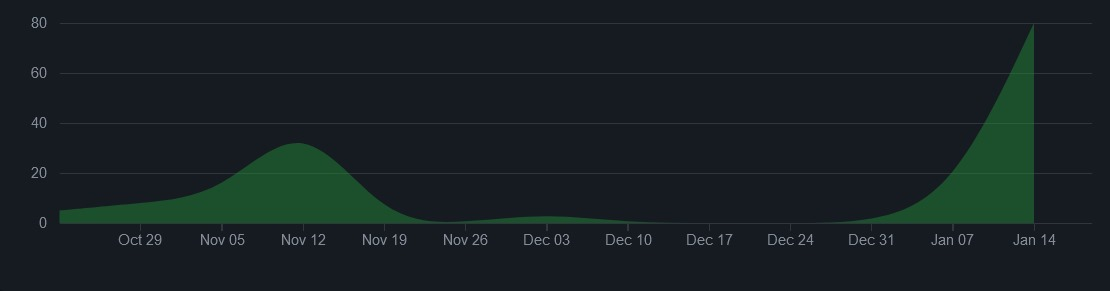
\includegraphics[width=\textwidth]{slike/main.JPG}
			\label{mainDiagram}
		\end{figure}
		
		\begin{figure}[H]
			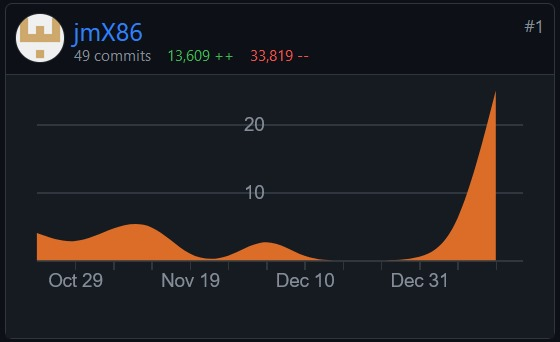
\includegraphics[width=\textwidth]{slike/josip.JPG}
			\label{josipDiagram}
		\end{figure}
	
		\begin{figure}[H]
			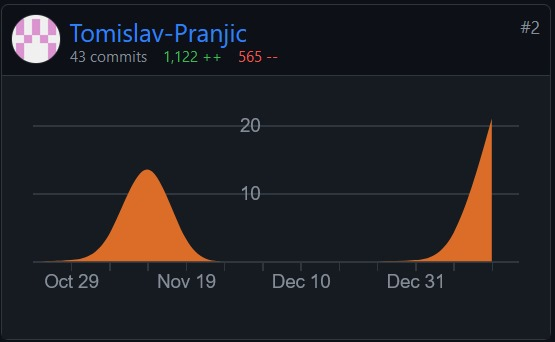
\includegraphics[width=\textwidth]{slike/tomislav.JPG}
			\label{tomiDiagram}
		\end{figure}
		
		\begin{figure}[H]
			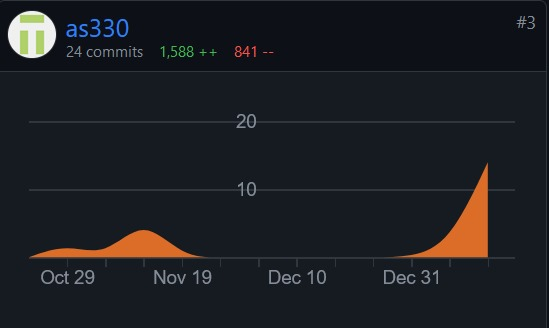
\includegraphics[width=\textwidth]{slike/ante.JPG}
			\label{anteDiagram}
		\end{figure}
		
		\begin{figure}[H]
			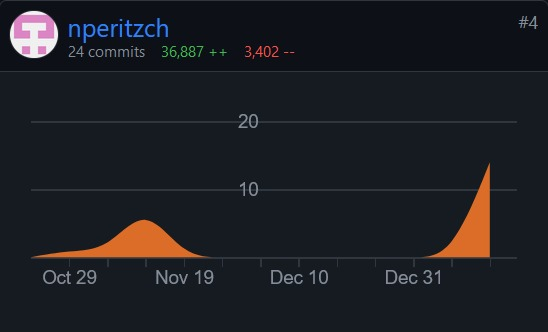
\includegraphics[width=\textwidth]{slike/nikola.JPG}
			\label{nikolaDiagram}
		\end{figure}
		
		\begin{figure}[H]
			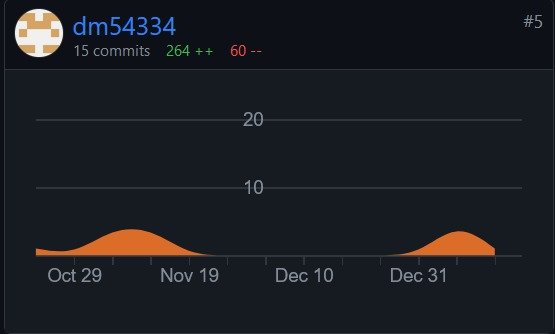
\includegraphics[width=\textwidth]{slike/diego.JPG}
			\label{diegoDiagram}
		\end{figure}
		
		\begin{figure}[H]
			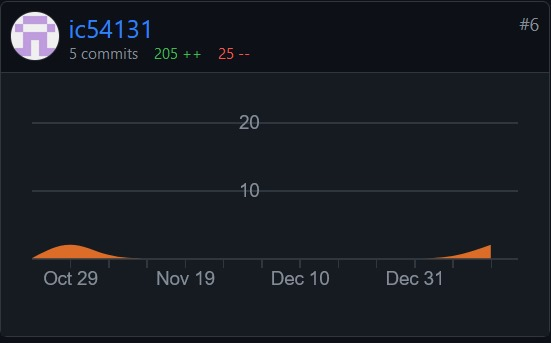
\includegraphics[width=\textwidth]{slike/ivan.JPG}
			\label{ivanDiagram}
		\end{figure}
		
		\begin{figure}[H]
			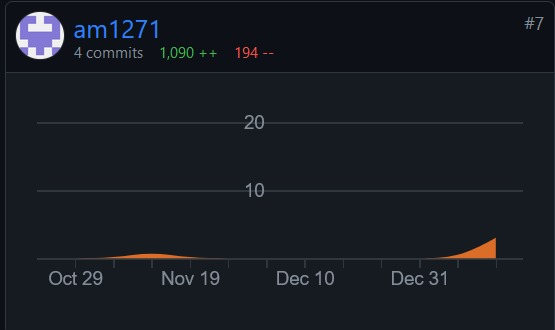
\includegraphics[width=\textwidth]{slike/antonija.JPG}
			\label{antonijaDiagram}
		\end{figure}
